\documentclass[11pt, a4paper]{article}

\usepackage{float}
\usepackage{amsmath}
\usepackage{graphicx,epsfig}
\usepackage{enumerate}
\usepackage[margin=.8in]{geometry}
\providecommand{\e}[1]{\ensuremath{\times 10^{#1}}}

\title{6.332 Final Project - 2.45GHz TLRCN Class E Resonant Rectifier}
\author{Josh Gordonson}

\begin{document}
\maketitle

\begin{center}
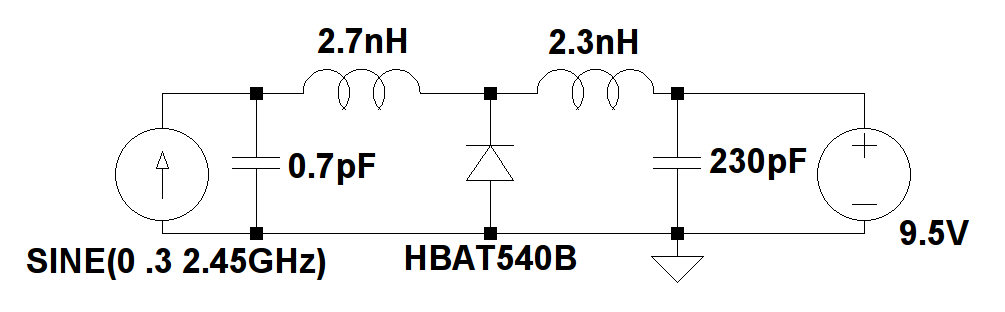
\includegraphics[width=.7\textwidth]{img/simple-schem.png}
\end{center}

\section{Class E Resonant Rectifiers}

Typical class E zero-voltage switching (ZVS), or low dv/dt, rectifiers are designed with a discrete ZVS shunt capacitance in parallel with the diode rectifier.
A large-valued LC filter makes the output look like a constant DC current source.  
While the diode is off, the ZVS capacitor provides a path for the mismatch in current between the input sinusoidal current source and the output current source.  
When the diode first turns off, the voltage across the diode and capacitor, $v_c=0$ and $\frac{dv_c}{dt}=0$.  
As the current through the capacitor begins to increase, the diode becomes more reverse-biased.  
Eventually, the current through the capacitor becomes negative, to the point where the voltage across the capacitor is zero again and the diode begins to conduct.  
Since the diode switches when $\frac{dv_c}{dt}=0$, there is little power lost during both the forward switching and reverse recovery transients \cite{kaz}.  
While the typical class E ZVS rectifier has nice output characteristics, its input impedance is far from resistive, due to the largely inductive output.  
By relaxing this constraint, Santiago-Gonzalez et al. have shown that it is possible to design a class E rectifier with a near-resistive input impedance over wide power ranges \cite{santiago}. \\

The relaxed rectifier design is resonant, where the output inductor $L_r$ and the diode shunt capacitance $C_r$ resonate while the diode is off.  
$C_r$ still maintains low $\frac{dv_c}{dt}$ switching, but the input impedance is much less reactive due to the smaller-valued $L_r$.  
The relaxed design operates in the same way as a typical class E rectifier, but the output inductor current ripple is larger.  
The current through $L_r$ resonates up while the diode is off and falls while the diode conducts.  \\

It can be shown that these two topologies will always look capacitive at the input.  
Analyzing the circuit in its two states is simply a matter of approximating the diode as a changing resistance.
In the on state the diode behaves like a near-short, providing a lot of damping to the parallel LC circuit.
In the off state the diode behaves like a near-open, providing almost no damping.
In both cases, the resonant frequency of the parallel LC circuit is lower than the operating frequency.
In the typical topology this is due to the large output inductor.
In the relaxed topology, driving the LC circuit below resonance causes the circuit to malfunction, so the resonant frequency must be chosen below the operating frequency.
Since $f_{op} > f_o$, the magnitude and phase will fall off as if connected to a purely capacitive circuit.  In other words, the input impedance has negative reactance. \\

In a typical rectifier, $C_r$ is a discrete component that absorbs the diode's parasitic capacitance \cite{santiago}.
In order to operate at UHF and mitigate component parasitics, this work uses the diode's parasitic capacitance as $C_r$.
The parasitic junction capacitance $C_{jo}$ of the HBAT540B is provided in Avago's datasheet as 3pF.\\

\section{Design Procedure}

The ideal value of $L_r$ can be determined by following the design procedure described by Santiago-Gonzalez et al \cite{santiago}.  
After selecting a diode (HBAT540B, $V_{r,peak}=33V$), resonant capacitance ($C_r=3pF$), and frequency of operation ($f=2.45GHz$), an output voltage $V_o=7.5V$ and maximum output power $P_{o,max}=1W$ can be chosen somewhat arbitrarily.  
From these values, the normalized capacitance is calculated:
\begin{equation*}
C_n=C_r\frac{2\pi f V_o^2}{P_{o,max}}=3pF \frac{2\pi\times2.45GHz\times7.5V^2}{1W}=2.6
\end{equation*}
This normalized capacitance is well off the plots provided, but extrapolating from Figure 5 in Santiago-Gonzalez et al, we find that for $C_n=2.6$, $L_n\approx0.3$, and:  
\begin{equation*}
L_r=L_n\frac{V_o^2}{2\pi fP_{o,max}}=1.1nH
\end{equation*}
Given this, spice simulations are needed to verify the results.

\begin{center}
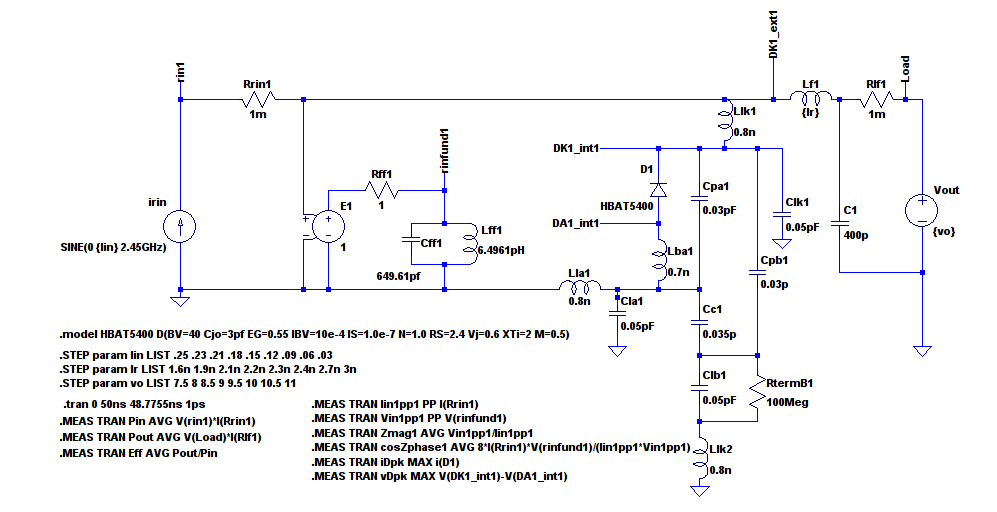
\includegraphics[width=.7\textwidth]{img/sim-schem.png}
\end{center}

Transient simulations were used to determine the input power, output power, efficiency, input resistance, input phase, and peak diode voltage while varying the input power, output voltage, and inductor value.
The approximated ideal inductance was off by about a factor of two, and the actual ideal inductor was found to be 2.3nH.  
The ideal output voltage was found to be 9.5V.

This produced an input impedance that varied from 20-180$\Omega$ over a 1W to .1W operating range with $12^\circ$ maximum phase.

\section{Results}
\subsection{Initial Results}

Settling on these parameters, a two-stage TLRCN board was designed to compress the 20-180$\Omega$ impedance down to 48-52$\Omega$.  
The board was fabricated with additional areas to calibrate out to the reference plane and to independently test the TLRCN and rectifier blocks.  
In addition to the aforementioned components, an output filter composed of three silver mica capacitors, values 1, 10, and 220pF was used to remove the current ripple effecs on the output voltage measurement.
An additional output capacitor, whose self-resonance was tuned to $\sim$2.45GHz was used to put a null at the operating frequency.
On the test bench, the isolated rectifier produced a minimum voltage standing wave ratio of 3 over the operating range.  
The input impedance was clearly not resistive.  

\subsection{Reactance Canceling}
To determine whether or not the reactance was positive or negative, a few values of shunt capacitance and inductance were applied to the input leg.  
All shunt capacitors made the VSWR higher, whereas some values of shunt inductance slightly decreased the VSWR.  
This implied that the input reactance was negative, which matches the theoretical capacitive operating point input impedance.  
To cancel the negative reactance, a series inductor was inserted between the TLRCN and the rectifier.  
With a 2.7nH series inductor, the VSWR dropped to a minimum of 1.8. 
Assuming the impedance mismatch is linear and purely reactive, there exists an inductance that cancels the reactance, dropping the VSWR to 1.
In practice, a small range of values of inductors were available (... 2nH, 2.2nH, 2.4nH, 2.7nH, ...), so it's unlikely that the correct value was used.  
In an attempt to trim down the reactance, a range of shunt capacitances were tested.  
A 0.7pF shunt capacitor resulted in a VSWR of 1.1.

\subsection{TLRCN Rectifier and Final Results}

The two-stage TLRCN Rectifier was constructed using the 0.7pF shunt capacitance and 2.7nH series inductance on each of the four resonant rectifiers.  
Testing over a power range of 0.4 to 4 watts (0.1 to 1 watt per rectifier), the efficiency per converter improved from 20\% to 50\% on the low end, while remaining about 70\% efficient on the high end.  
The standing wave ratio remained under 1.3 for the enitre power range.
The TLRCN clearly functioned as intended, compressing the mostly resistive input impedance of 20-180$\Omega$ down to $\sim$48-52$\Omega$, resulting in better matching between the source and rectifier input.

\section{Future Work}


\begin{thebibliography}{1}
\bibitem{kaz} M.K. Kazimierczuk, {\em “Analysis of Class E Zero-Voltage-Switching Rectifier,”} IEEE Transactions on Circuits and Systems, vol.37, no.6, pp.747-755, June 1990. \\
\bibitem{santiago} Juan A. Santiago-González, Khurram K. Afridi and David J. Perreault, {\em "Design of Resistive-Input Class E Resonant Rectifiers for Variable-Power Operation,"} IEEE 14th COMPEL, June 2013. \\
\end{thebibliography}
\end{document}

